\documentclass{article}
\usepackage[utf8]{inputenc}
\usepackage{titling}
\usepackage{graphicx}
\usepackage{xcolor}
\usepackage[colorlinks=true,linkcolor=darkgray]{hyperref}
\usepackage[spanish]{babel}


\title{Criptografía (Parte 4)}
\author{Cristina Díaz García}
\date{November 2018}

\renewcommand\maketitlehooka{\null\mbox{}\vfill}
\renewcommand\maketitlehookd{\vfill\null}


\begin{document}

\addcontentsline{toc}{section}{Índice general}

\begin{titlingpage}
\maketitle
\end{titlingpage}

\newpage

\tableofcontents

\newpage

\section{Ejercicio 1}
\subsection{Apartado a}
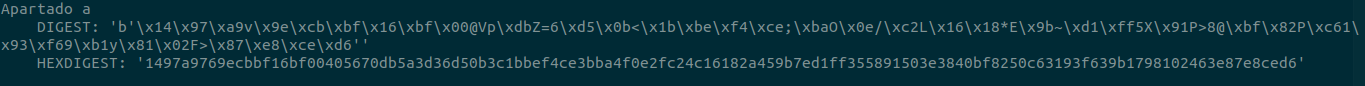
\includegraphics[scale=0.3]{ApartadoA.png} 

\subsection{Apartado b}
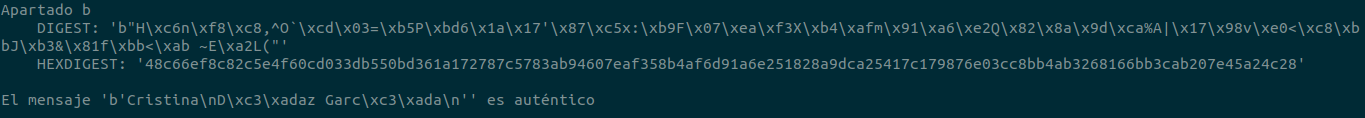
\includegraphics[scale=0.3]{ApartadoB.png}

\subsection{Apartado c}
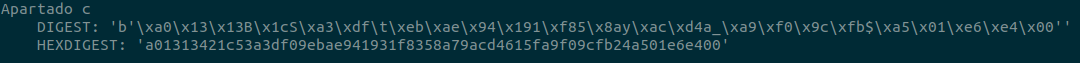
\includegraphics[scale=0.4]{ApartadoC.png}

\newpage

\section{Ejercicio 2}
\textbf{\textit{SHA-2 family}} es compatible con \textit{HMAC}, 
\textbf{\textit{SHA-3 family}} no es compatible porque no tiene el parametro \textit{block\_size}, 
\textbf{\textit{BLAKE2}} no es compatible porque no se puede establecer el \textit{digest\_size} cuando se usa \textit{HMAC}.

\end{document}